\section{Data and theory}
\label{sec:theory}

In this work, the photon
content of the proton $\gamma(x,Q^2)$ will be extracted from a PDF analysis based
on the legacy inclusive structure function data combination from HERA~\cite{Abramowicz:2015mha}
supplemented by the ATLAS measurements of the high-mass Drell-Yan process
at $\sqrt{s}=8$ TeV~\cite{Aad:2016zzw}.
%
The HERA structure functions are the backbone of all
recent PDF fits, providing information on the quark/antiquark and gluon content of 
the proton, while the high-mass Drell-Yan data provide
direct sensitivity to the photon PDF.
%
Indeed, dilepton production at the Born level can arise  from either quark-antiquark $s$-channel
scattering or from photon-photon $t$-channel scattering mediated by a lepton,
as shown in Fig.~\ref{fig:photoninduced}.

%%%%%%%%%%%%%%%%%%%%%%%%%%%%%%%%%%%%%%%%%%%%%%%%%%%%%%%%%%%%%%%%
\begin{figure}[h]
  \begin{center}
    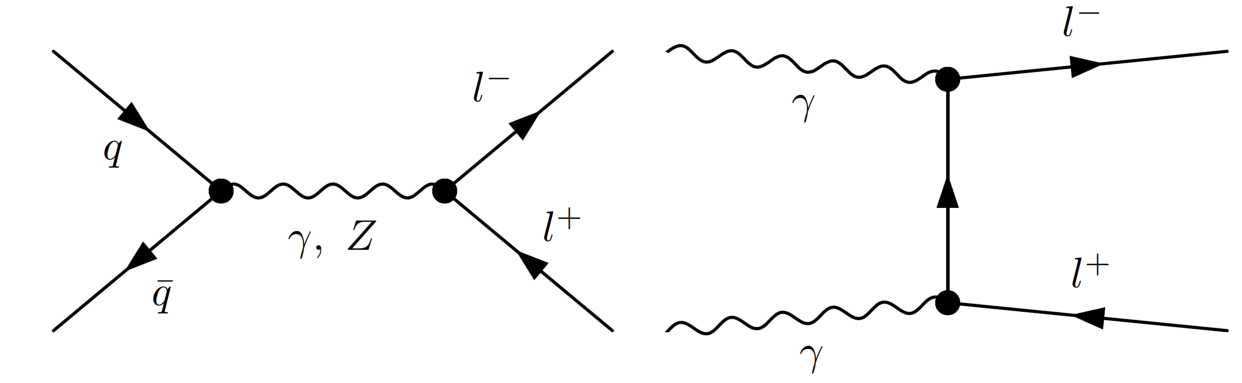
\includegraphics[width=8cm]{plots/photoninduced.pdf}
    \end{center}
  \caption{Two of the processes that contribute to lepton-pair
  production at hadron colliders at the Born level.}
\label{fig:photoninduced}
\end{figure}
%%%%%%%%%%%%%%%%%%%%%%%%%%%%%%%%%%%%%%%%%%%%%%%%%%%%%%%%%%%%%%%%

Deep-inelastic structure functions and PDF evolution will be performed
with the program {\tt APFEL}~\cite{Bertone:2013vaa}, which in its latest
version is accurate up to NNLO for the QCD corrections and up to
NLO for the QED corrections, as described in appendix~\ref{sec:appendixAPFEL}.
%
To be precise, this means that the DGLAP evolution equations are solved including
the splitting functions $P(\alpha_s,\alpha)$ up to $\mathcal{O}\lp \alpha_s^3\rp$ in the QCD
coupling and up to $\mathcal{O}\lp \alpha_s\alpha\rp$ in the QED coupling,
and that DIS coefficient functions include corrections up to $\mathcal{O}\lp \alpha_s^2\rp$
in QCD and up to $\mathcal{O}\lp \alpha^2\rp$ in QED.
%
Heavy quark (charm and bottom) mass effects in DIS structure functions are accounted
for using the FONLL-B(C) general-mass scheme~\cite{Forte:2010ta}
for the NLO (NNLO) fits.
%
As for the numerical values of the heavy quark masses in the pole scheme,
we take  $m_c=1.47~$GeV and $m_b=4.5~$GeV, consistent with the latest PDG average.
%
The strong (QED) coupling constant is chosen to be  $\alpha_s(m_Z)=0.118$~\cite{PDG}
($\alpha(m_Z)=1/127$).
%
Let us recall that heavy quark structure functions with running masses
are also implemented in {\tt APFEL}~\cite{Bertone:2016ywq},
though their use should not lead to any difference for the determination of the photon PDF.
 
Concerning the high-mass Drell-Yan cross-sections,
both the contributions can be 
simulated with {\tt MadGraph5{\_}aMC@NLO}~\cite{Alwall:2014hca}
(version 2.4.3) and interfaced to {\tt APPLgrid}~\cite{Carli:2010rw}
v01-04-70) and {\tt aMCfast}~\cite{Carli:2010rw} (version 01-03-00).
%
A special release of {\tt APPLgrid} is used to account for the photon PDF within the proton {\it need references for the programs}.
Both contributions are generated in the 5-flavour scheme, where all the quarks, except for the \textit{top}
 quark, are treated as massless quarks; all the calculations are performed at fixed-order (FO) without 
 parton showers.



Theoretical predictions for both the one-dimensional $\frac{d\sigma}{dm_{ll}}$ distribution 
(where $m_{ll}$ is the invariant mass of the dilepton pair in the final state) and the double-differential 
distributions $\frac{d^{2}\sigma}{dm_{ll}d|y_{ll}|}$ (where $|y_{ll}|$ is the rapidity of the dilepton pair) 
and $\frac{d^{2}\sigma}{dm_{ll}\Delta\eta_{ll}}$ (where $\Delta\eta_{ll}$ represents the difference in 
pseudorapidity between the two leptons) are generated for both the electron and the muon channels.
 
These predictions are generated using the same selections as in reference~\cite{jhep08-2016-009}
as follows:
\begin{itemize}
\item the invariant mass of the lepton pair is required to be greater than 116 GeV;
\item the absolute value of the pseudorapidity of each lepton is required to be less than 2.5;
\item the transverse momentum ($p_{T}$) of the leading lepton has to be greater than 40 GeV;
\item the $p_{T}$ of the sub-leading lepton has to be greater than 30 GeV.
\end{itemize} 
The binning used is the same as used in reference~\cite{jhep08-2016-009}. For the invariant mass 
distribution, there are 12 bins between 116 GeV and 1.5 TeV with variable bin widths; and for both of the 
 the two-dimensional distributions, there are five different histograms, each one for a different invariant
 mass range: (a) 116 GeV < $m_{ll}$ < 150 GeV; (b) 150 GeV < $m_{ll}$ < 200 GeV; (c) 200 GeV < $m_{ll}$ < 300 GeV; (d) 300 GeV < $m_{ll}$ < 500 GeV; (e) 500 GeV < $m_{ll}$ < 1500 GeV.
 The APPLgrids for the first three $m_{ll}$ intervals are divided into 12 bins with fixed bin 
width between $|y_{ll}^{mim}|$ ($|\Delta\eta_{ll}|$)  = 0.0 (0.0) and $|y_{ll}^{max}|$ ($|\Delta\eta_{ll}|$) = 2.4 (3.0), while the final two $m_{ll}$ intervals are divided into 6 bins with fixed bin width scanning the same $|y_{ll}|$ and $|\Delta\eta_{ll}|$ ranges.

Dynamical renormalization ($\mu_{R}$) and factorization ($\mu_{R}$) scales are used in the calculations 
and both are set to $m_{ll}$. The theoretical calculations were validated by comparing both the NLO QCD + LO EW predictions and the 
LO PI predictions to those computed using the FEWZ 3.1 framework. These calculations are evaluated in the $G_{F}$ electroweak scheme, with the following values for the couplings:
 $\alpha_{S}$ = 0.118; $1/\alpha_{EW}$ = 1/127. The difference between the two predictions is at most 1${\%}$, for both the 1-dimensional and the 2-dimensional distributions.

In order to make a next-to-next-to-leading order (NNLO) fit k-factors ($k_{F}$) are computed matching
 the NLO QCD + LO EW cross sections to higher order (HO) calculations. These are computed using 
FEWZ, with the same input parameters as for the NLO computations. The $k_{F}$ are defined as:
\begin{equation}
k_{F}=\frac{NNLO\  QCD  + NLO\  EW \sigma}{NLO\  QCD + LO\  EW \sigma}
\end{equation}
The MMHT2014NNLO PDF set is used to compute both numerator and denominator.
 The $k_{F}$ are close to the unity and their variation is $\sim 2\%$. {\it provide Table of Final k-factors?}


Discuss theory improvements: addition of the NLO QED+QCD piece 
